\documentclass[halfparskip]{beamer}


\mode<presentation>
{
  \usetheme{CambridgeUS}
  \usecolortheme{crane}
 
  \setbeamercovered{transparent}
}


\usepackage[ngerman]{babel}
\usepackage{enumitem}
\usepackage[T1]{fontenc}
\usepackage{graphicx}
\usepackage[utf8x]{inputenc}
\usepackage{lmodern}
\usepackage{tabularx}
\usepackage{amssymb}
\usepackage{pifont}
\newcommand{\cmark}{\ding{51}}
\newcommand{\xmark}{\ding{55}}

\title{Crawling von Datenschutzerklärung-Historien}
\subtitle{Zwischenpräsentation}

\author[AP, JHD, SK]{Alexander Prull, Jörn-Henning Daug, Simon Kaleschke}

\institute{Universität Leipzig}

\date[16. 12. 2016]{16. Dezember 2016}

\subject{Crawling von Datenschutzerklärung-Historien}

\AtBeginSection[]
{
  \begin{frame}<beamer>{Gliederung}
    \tableofcontents[currentsection,currentsubsection]
  \end{frame}
}

\begin{document}

\begin{frame}
  \titlepage
\end{frame}

\begin{frame}{Gliederung}
  \tableofcontents
\end{frame}

\section{Projektbeschreibung}
\begin{frame}{Projektbeschreibung}
	\begin{block}{Motivation}
	\begin{itemize}[label=$\bullet$]
	\item Aktuell geltende DSEs analysieren.
	\item Die Entwicklungsgeschichte von DSEs betrachten.
	\item Trends und Veränderungen beobachten.
	\end{itemize}
	\end{block}
	\begin{block}{Aufgaben}
		\begin{itemize}[label=$\bullet$]
			\item DSEs (täglich) extrahieren.
			\item Diese geeignet anzeigen.
			\item Unterschiede über Zeit darstellen.
		\end{itemize}
	\end{block}
	{\tiny DSE = Datenschutzerklärung}
\end{frame}

\section{Lösungsansatz}
\begin{frame}{Lösungsansatz}
	\begin{block}{Aufteilung}
		\begin{itemize}[label=$\bullet$]
			\item Extraktion: Ruby, XPath, SQLite.
			\item Backend: Java, REST-Services.
			\item Frontend: HTML5, CSS3, JavaScript, AngularJS, Bootstrap.
		\end{itemize}
	\end{block}
	\begin{block}{Arbeitspakete}
		\begin{itemize}[label=$\bullet$]
			\item Recherche (100 \%)
			\item Grundgerüst (100 \%)
			\item Feinschliff (80 \%)
		\end{itemize}
	\end{block}
\end{frame}

\section{Softwarearchitektur}
\begin{frame}{Extraktion}
	\centering
	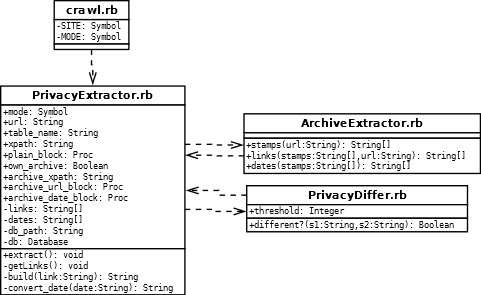
\includegraphics[scale=0.5]{extraction.png}
\end{frame}
\begin{frame}{Backend}
	\centering
	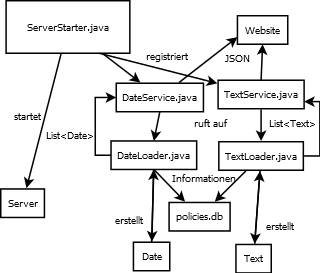
\includegraphics[scale=0.3]{backend.png}
\end{frame}
\begin{frame}{Frontend}
	\centering
	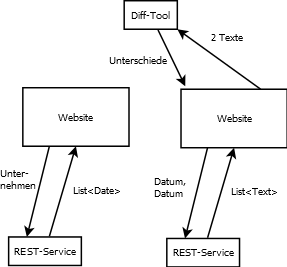
\includegraphics[scale=0.75]{frontend.png}
\end{frame}
\begin{frame}{Datenbankstruktur}
	\begin{block}{Die SQLite-Datenbank hat folgende Spalten:}
		\begin{tabularx}{\textwidth}{|r|X|}
			\hline
			\textbf{Spalte} & \textbf{Bedeutung} \\ \hline \hline
			ID & Primärschlüssel. \\ \hline
			SYSTEM\_DATE & Datum, an dem die Datenschutzhistorie in dem aktuellen Zustand war.\\ \hline
			DISPLAY\_DATE & Gleiches Datum in benutzerfreundlicher Schreibweise. \\ \hline
			LINK & Hyperlink, wo die extrahierte Historie zu finden ist.\\ \hline
			CONTENT & Der extrahierte Plaintext.\\ \hline
		\end{tabularx}
	\end{block}
\end{frame}

\section{Ergebnisse}
\begin{frame}{Übersicht gecrawlte Webseiten}
	\begin{block}{}
		\begin{tabularx}{\textwidth}{|r|c|c|c|X|}
			\hline
			\textbf{Firma} & \textbf{Archiv} & \textbf{Versionen} & \textbf{Zeitspanne} & \textbf{Qualität} \\ \hline \hline
			Alternate & \xmark & 7 & 08/2014 - 07/2016 &  0.9 \\ \hline
			Amorelie & \xmark & 11 & 01/2013 - 10/2016 &  0.7 \\ \hline
			Apple & \xmark & 12 & 09/2014 - 09/2016 &  1.0 \\ \hline
			Burgerking & \xmark & 2 & 02/2015 - 12/2016 &  0.7 \\ \hline
			Edeka & \xmark & 4 & 11/2014 - 10/2016 &  0.7 \\ \hline
			Google & \cmark & 22 & 06/1999 - 01/2017 &  0.8 \\ \hline
			Microsoft & \xmark & 7 & 02/2016 - 01/2017 &  0.9 \\ \hline
			Payback & \xmark & 10 & 09/2011 - 10/2016 &  0.9 \\ \hline
			Paypal & \xmark & 2 & 04/2014 - 11/2016 &  0.9 \\ \hline
			RocketbeansTV & \xmark & 4 & 10/2014 - 09/2016 &  1.0 \\ \hline
		\end{tabularx}
	\end{block}
\end{frame}
\begin{frame}{Übersicht gecrawlte Webseiten}
	\begin{block}{}
		\begin{tabularx}{\textwidth}{|r|c|c|c|X|}
			\hline
			\textbf{Firma} & \textbf{Archiv} & \textbf{Versionen} & \textbf{Zeitspanne} & \textbf{Qualität} \\ \hline \hline
			Steam & \xmark & 3 & 09/2012 - 11/2016 &  0.8 \\ \hline
			Subway & \xmark & 3 & 05/2016 - 10/2016 &  0.9 \\ \hline
			Süddeutsche & \xmark & 1 & 04/2015 - 04/2015 &  0.2 \\ \hline
			Trivago & \xmark & 1 & 04/2016 - 04/2016 &  0.7 \\ \hline
			Twitter & \cmark & 10 & 05/2007 - 01/2016 &  0.8 \\ \hline
			Uni Leipzig & \xmark & 1 & 06/2013 - 06/2013 &  0.5 \\ \hline
			Vine & \xmark & 5 & 03/2013 - 01/2017 &  1.0 \\ \hline
			WhatsApp & \cmark & 2 & 07/2012 - 01/2017 &  0.9 \\ \hline
			Wikimedia & \cmark & 4 & 06/2006 - 06/2014 &  1.0 \\ \hline
			Zalando & \xmark & 3 & 09/2010 - 11/2012 &  0.9 \\ \hline
		\end{tabularx}
	\end{block}
\end{frame}

\end{document}
